\chapter{Data Flow}

% \begin{figure}[h]
    \begin{center}
    % 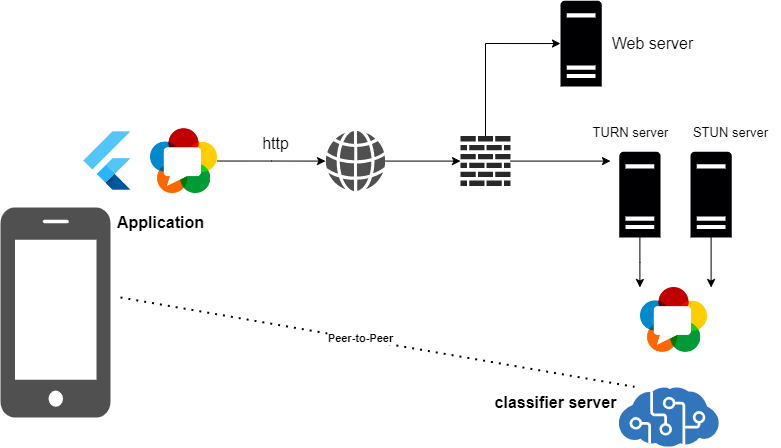
\includegraphics{pic/webrtc.png}
    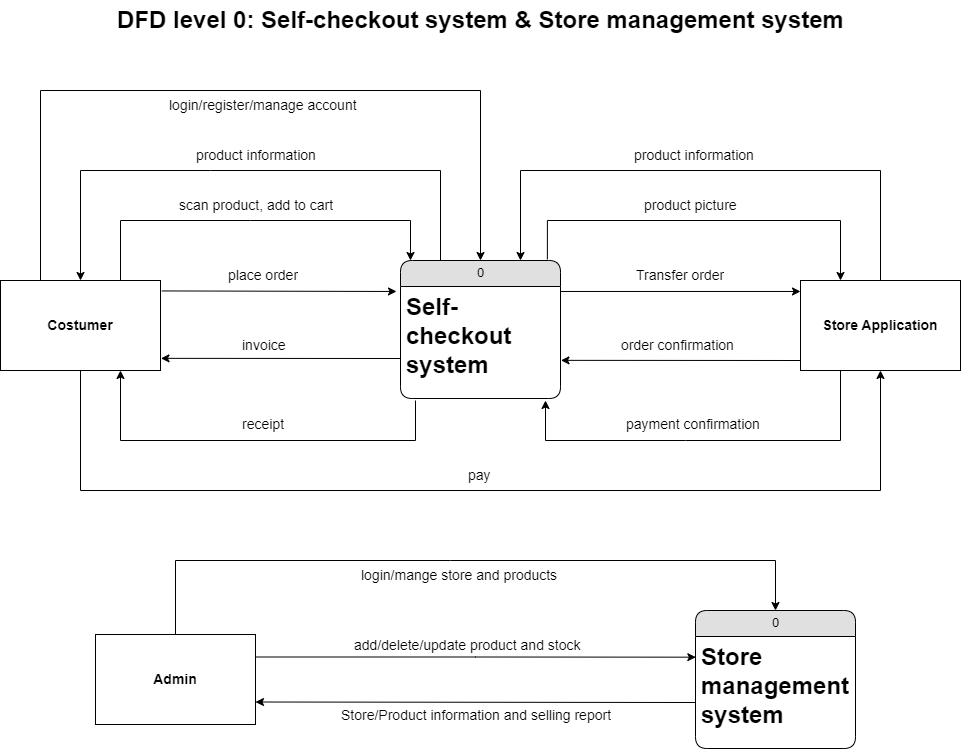
\includegraphics[scale=0.25]{pic/dataflow_p1.png}\\
    \vspace{2cm}
    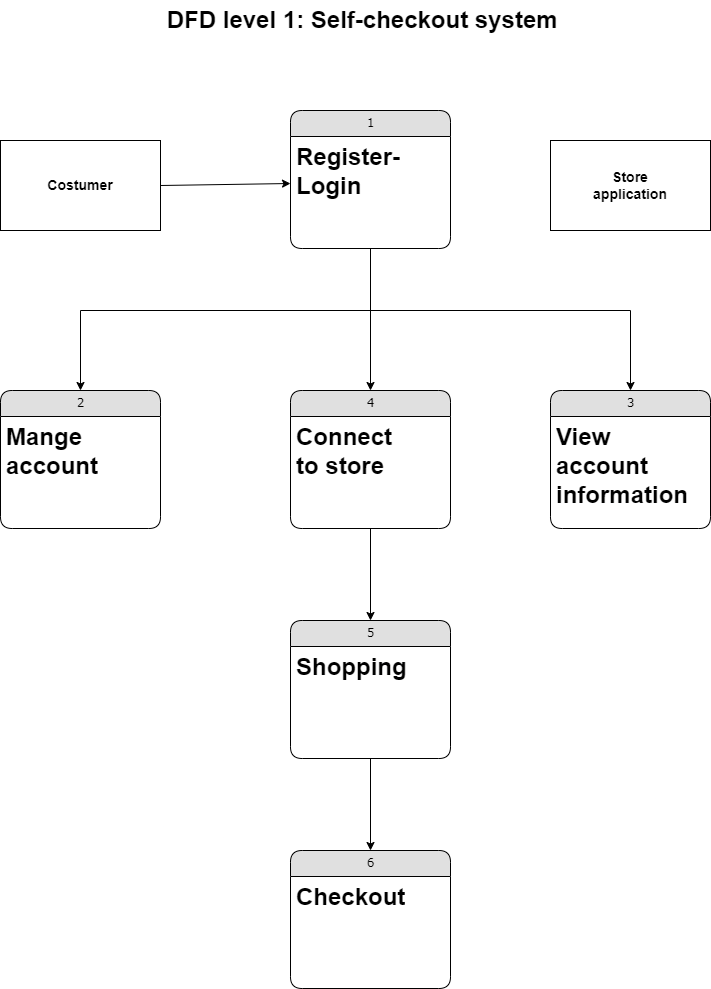
\includegraphics[scale=0.25]{pic/dataflow_p2.png}
    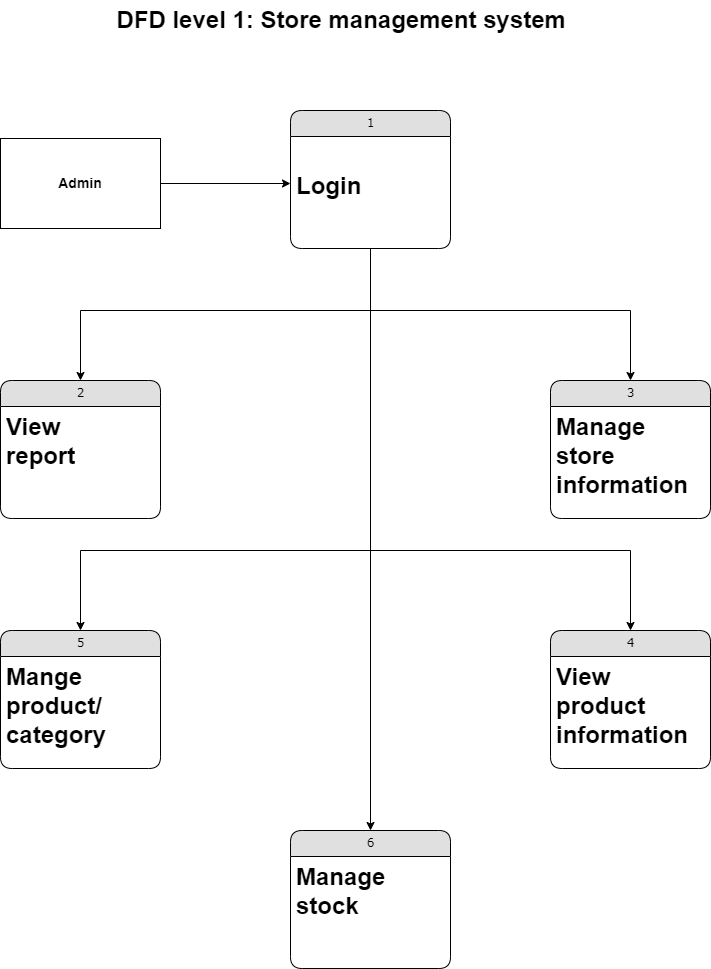
\includegraphics[scale=0.25]{pic/dataflow_p3.png}
    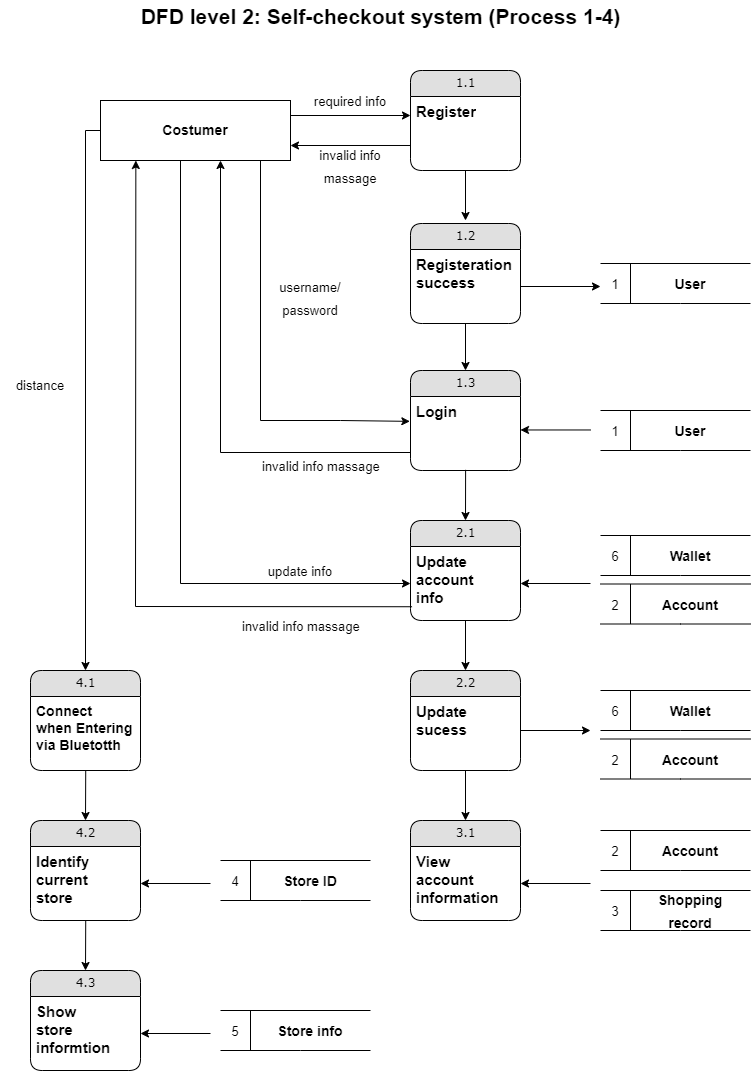
\includegraphics[scale=0.25]{pic/dataflow_p4.png}
    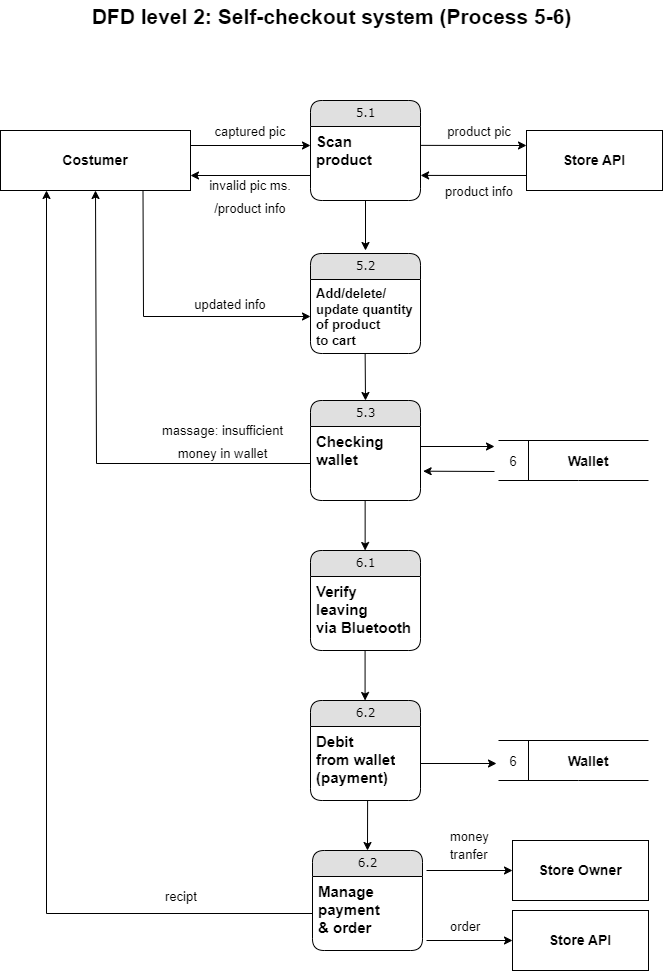
\includegraphics[scale=0.25]{pic/dataflow_p5.png}\\
    \vspace{2cm}
    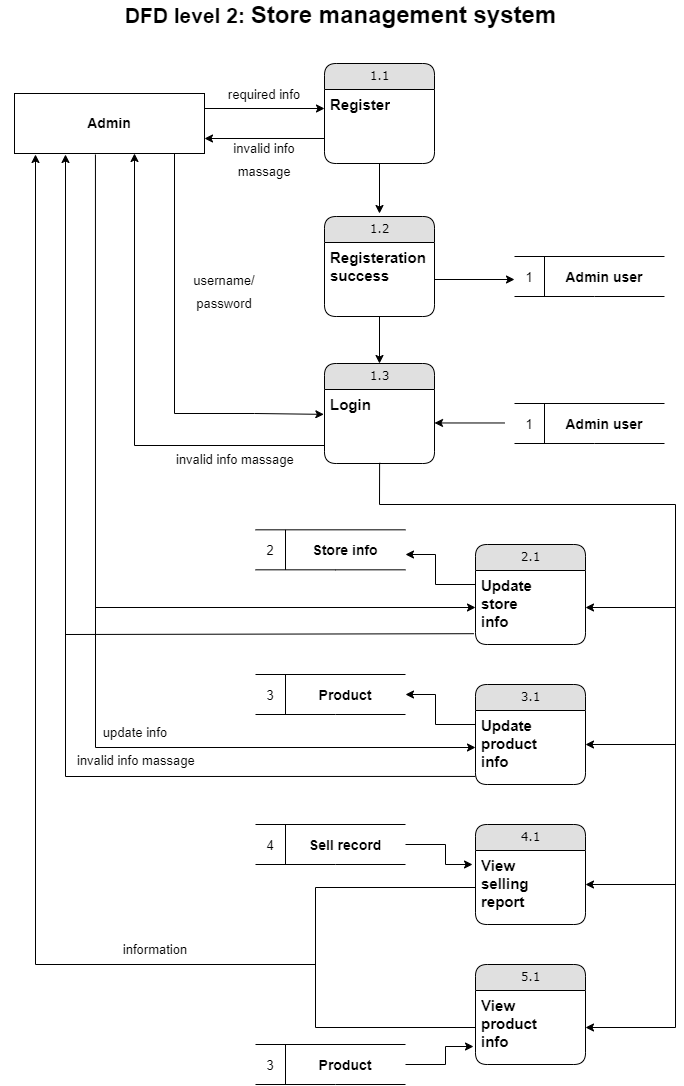
\includegraphics[scale=0.25]{pic/dataflow_p6.png}


    \begin{figure}[h]
        \begin{center}
        % 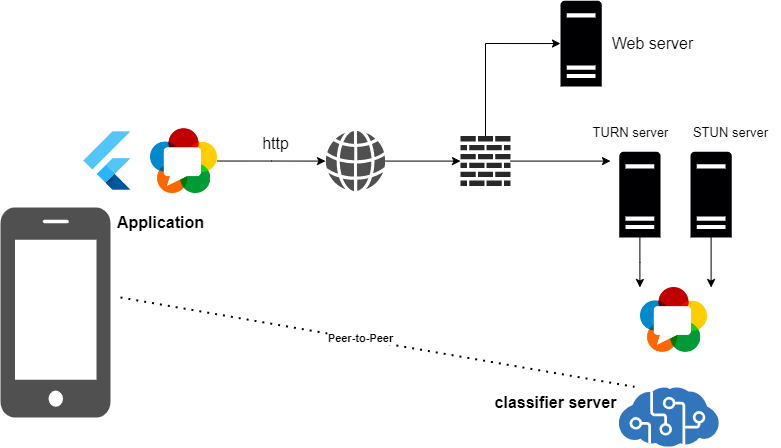
\includegraphics{pic/webrtc.png}
        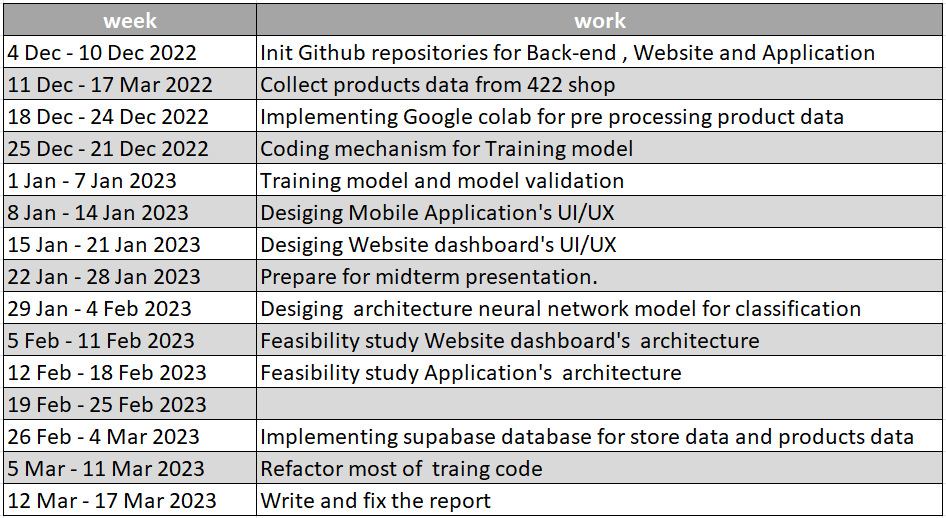
\includegraphics[scale=0.5]{pic/work_plane.png}
        \end{center}
        
        \caption[Work table]{Work table}
        \label{fig:Work table}
        \end{figure}
     


    \end{center}
    
    % \caption[Data Flow Diagram all]{Data Flow Diagram all}
    % \label{fig:Data Flow Diagram all}
    % \end{figure}

% \section{Appendix section}

% Text for a section in the first appendix goes here.

% test ทดสอบฟอนต์ serif ภาษาไทย

% \textsf{test ทดสอบฟอนต์ sans serif ภาษาไทย}

% \verb+test ทดสอบฟอนต์ teletype ภาษาไทย+

% \texttt{test ทดสอบฟอนต์ teletype ภาษาไทย}

% \textbf{ตัวหนา serif ภาษาไทย \textsf{sans serif ภาษาไทย} \texttt{teletype ภาษาไทย}}

% \textit{ตัวเอียง serif ภาษาไทย \textsf{sans serif ภาษาไทย} \texttt{teletype ภาษาไทย}}

% \textbf{\textit{ตัวหนาเอียง serif ภาษาไทย \textsf{sans serif ภาษาไทย} \texttt{teletype ภาษาไทย}}}

% \url{https://www.example.com/test_ทดสอบ_url}

% \chapter{\ifenglish Manual\else คู่มือการใช้งานระบบ\fi}

% Manual goes here.
